%%%%%%%%%%%%%%%%%%%%%%%%%%%%%%%%%%%%%%%%%%%%%%%%%%%%%%%%%%%%%%%%%%%%%%%%%%%%%%%%

\section{Haute disponibilité (HA)}

%%%%%%%%%%%%%%%%%%%%%%%%%%%%%%%%%%%%%%%%%%%%%%%%%%%%%%%%%%%%%%%%%%%%%%%%%%%%%%%%

\begin{frame}[fragile]{Solutions de HA}

   \begin{itemize}
      \item Il existe plusieurs solutions de HA.
      \item Certaines solutions intègrent nativement le partitionnement de données.
      \item Citus fait partie des solutions HA avec partitionnement de données
      \item L'objectif de cette formation est de permettre au client d'administrer ses bases de données avec le choix des outils qu'il a réalisé
      \item Le choix réalisé est \textbf{repmgr}
   \end{itemize}

\begin{toile}
\toileurl{https://docs.citusdata.com/en/v11.2/get\_started/what\_is\_citus.html}
\toileurl{https://repmgr.org/}
\end{toile}

\end{frame}

%%%%%%%%%%%%%%%%%%%%%%%%%%%%%%%%%%%%%%%%%%%%%%%%%%%%%%%%%%%%%%%%%%%%%%%%%%%%%%%%

\begin{frame}[fragile]{Présentation de \textbf{repmgr}}

   \begin{itemize}
      \item repmgr est une solution de gestion de:
         \begin{itemize}
            \item la réplication
            \item le switchover
            \item et le failover PostgreSQL
         \end{itemize}
      \item Elle supporte les versions PostgreSQL de 9.4 à 15
      \item Elle est portée par l'entreprise EDB
   \end{itemize}

\end{frame}

%%%%%%%%%%%%%%%%%%%%%%%%%%%%%%%%%%%%%%%%%%%%%%%%%%%%%%%%%%%%%%%%%%%%%%%%%%%%%%%%

\begin{frame}[fragile]{Caractéristiques avancées de \textbf{repmgr}}

   \begin{itemize}
      \item repmgr intègre les nouveautés introduites par PostgreSQL 9.3:
         \begin{itemize}
            \item la réplication en cascade
            \item la commutation de la ligne de temps (timeline switching)
            \item et la sauvegarde de base via la réplication
         \end{itemize}
      \item Il est disponible sous la licence GPLv3
      \item La dernière version disponible pendant la rédaction de ce document est la v5.3.3
   \end{itemize}

\end{frame}

%%%%%%%%%%%%%%%%%%%%%%%%%%%%%%%%%%%%%%%%%%%%%%%%%%%%%%%%%%%%%%%%%%%%%%%%%%%%%%%%

\section{Partitionnement des données}

%%%%%%%%%%%%%%%%%%%%%%%%%%%%%%%%%%%%%%%%%%%%%%%%%%%%%%%%%%%%%%%%%%%%%%%%%%%%%%%%

\begin{frame}[fragile]{Présentation des indexes B-Tree}

   \begin{itemize}
      \item Un index de type B-Tree est un arbre composé:
      \begin{itemize}
         \item d'une racine
         \item de noeuds intermédiaires
         \item de feuilles
      \end{itemize}
      \item Les feuilles correspondent aux données dans les tables
      \item Chaque noeud intermédiaire porte un nombre de \textbf{clefs} maximum et minimum
      \item Les \textbf{clés} définissent les bornes minimum et maximum des valeurs portées par les noeuds enfants
      \item Lorsqu'un noeud atteint son nombre maximum d'enfants, une scission ("split") a lieu
      \item Lorsqu'un noeud atteint son nombre minimum d'enfants, une fusion ("merge") a lieu

   \end{itemize}

\begin{toile}
\toileurl{https://en.wikipedia.org/wiki/B-tree}
\toileurl{https://www.postgresql.org/docs/15/btree.html}
\toileurl{https://www.postgresql.org/docs/15/btree-implementation.html}
\end{toile}

\end{frame}

%%%%%%%%%%%%%%%%%%%%%%%%%%%%%%%%%%%%%%%%%%%%%%%%%%%%%%%%%%%%%%%%%%%%%%%%%%%%%%%%

\begin{frame}[fragile]{L'objectif des indexes B-Tree}

   \begin{itemize}
      \item L'objectif de l'index B-Tree est de stocker en mémoire une partie d'un index très volumineux
      \item Cet objectif est atteint par le fait que les noeuds intermédiaires indexent des plages de données
   \end{itemize}

\end{frame}

%%%%%%%%%%%%%%%%%%%%%%%%%%%%%%%%%%%%%%%%%%%%%%%%%%%%%%%%%%%%%%%%%%%%%%%%%%%%%%%%

\begin{frame}[fragile]{Schéma explicatif des indexes B-Tree}

\begin{figure}
\begin{center}
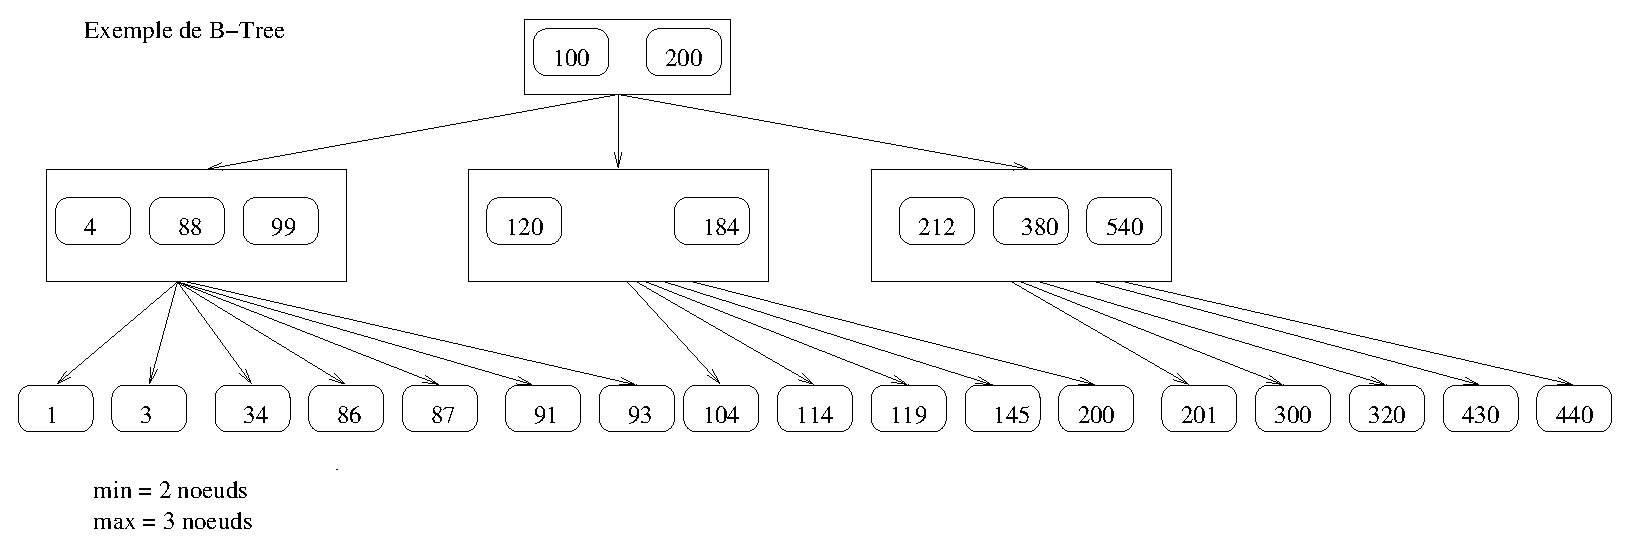
\includegraphics[angle=0, width=0.5\textwidth]{images/b_tree.eps}
\end{center}
\end{figure}

\end{frame}

%%%%%%%%%%%%%%%%%%%%%%%%%%%%%%%%%%%%%%%%%%%%%%%%%%%%%%%%%%%%%%%%%%%%%%%%%%%%%%%%

\begin{frame}[fragile]{Tables partitionnées}

   \begin{itemize}
      \item PostgreSQL supporte le partitionnement de données.
      \item Le partitionnement PostgreSQL consiste à découper une table logique en plusieurs petits morceaux physiques

   \end{itemize}

\begin{toile}
\toileurl{https://www.postgresql.org/docs/15/ddl-partitioning.html}
\end{toile}

\end{frame}

%%%%%%%%%%%%%%%%%%%%%%%%%%%%%%%%%%%%%%%%%%%%%%%%%%%%%%%%%%%%%%%%%%%%%%%%%%%%%%%%

\begin{frame}[fragile]{Tables partitionnées}

   \begin{itemize}
      \item Dans certaines situations, le partitionnement a plusieurs avantages:
      \begin{itemize}
         \item lorsque les données accédées sont localisées dans une partition ou un nombre réduit de partitions. A ce moment, la partie haute des indexes (B-Tree) qui correspond à ces données est entièrement en cache.
         \item lorsque les données modifiées ou accédée couvrent la majorité de la partition, il est préférable d'utiliser un scan séquentiel au lieu d'utiliser un index
         \item les chargements de données massifs ou suppressions massives de données correspondant à une partition sont réalisés en ajoutant une partition ou en supprimant une partition. En cas de suppression massive, un \textbf{VACUUM} est économisé
         \item les données ou partitions les moins utilisées peuvent être migrées vers des disques moins onéreux et moins rapides
      \end{itemize}

   \end{itemize}

\end{frame}

